\documentclass[border=10pt]{standalone}
\usepackage{tikz}
\usepackage[T1]{fontenc}
\usepackage{rubfonts2009}
% FIXME: Blue should be #003560, but that'd conflict with the front page colors
\definecolor{rubblue}{HTML}{003660}
\definecolor{rubgreen}{HTML}{8dae10}
\definecolor{rubgray}{HTML}{e7e7e7}
\usetikzlibrary{%
    shapes.geometric,
    shapes.misc,
    trees,
    positioning,
}
\makeatletter
\newcount\dirtree@lvl
\newcount\dirtree@plvl
\newcount\dirtree@clvl
\def\dirtree@growth{%
  \ifnum\tikznumberofcurrentchild=1\relax
  \global\advance\dirtree@plvl by 1
  \expandafter\xdef\csname dirtree@p@\the\dirtree@plvl\endcsname{\the\dirtree@lvl}
  \fi
  \global\advance\dirtree@lvl by 1\relax
  \dirtree@clvl=\dirtree@lvl
  \advance\dirtree@clvl by -\csname dirtree@p@\the\dirtree@plvl\endcsname
  \pgf@xa=2mm\relax
  \pgf@ya=-1cm\relax
  \pgf@ya=\dirtree@clvl\pgf@ya
  \pgftransformshift{\pgfqpoint{\the\pgf@xa}{\the\pgf@ya}}%
  \ifnum\tikznumberofcurrentchild=\tikznumberofchildren
  \global\advance\dirtree@plvl by -1
  \fi
}
\tikzset{%
    base/.style = {
        minimum height=0.75cm,
        text centered,
        font=\fontfamily{rubflama}\selectfont,
        line width=0.1mm,
        anchor=west,
    },
    doc/.style = {
        base,
        rounded rectangle,
        fill=rubgray,
    },
    element/.style = {
        base,
        chamfered rectangle,
        fill=rubgreen,
    },
    textnode/.style = {
        base,
        rectangle,
        text=white,
        fill=rubblue,
    },
    cdata/.style = {
        base,
        rectangle,
        text=white,
        fill=rubblue!80,
    },
    comment/.style = {
        base,
        rectangle,
        fill=rubgray!80!black,
    },
    pi/.style = {
        base,
        rectangle,
        fill=rubgreen!40,
    },
    growth function=\dirtree@growth,
    edge from parent path={
        (\tikzparentnode.south) |- (\tikzchildnode.west)
    }
}
\makeatother
\begin{document}
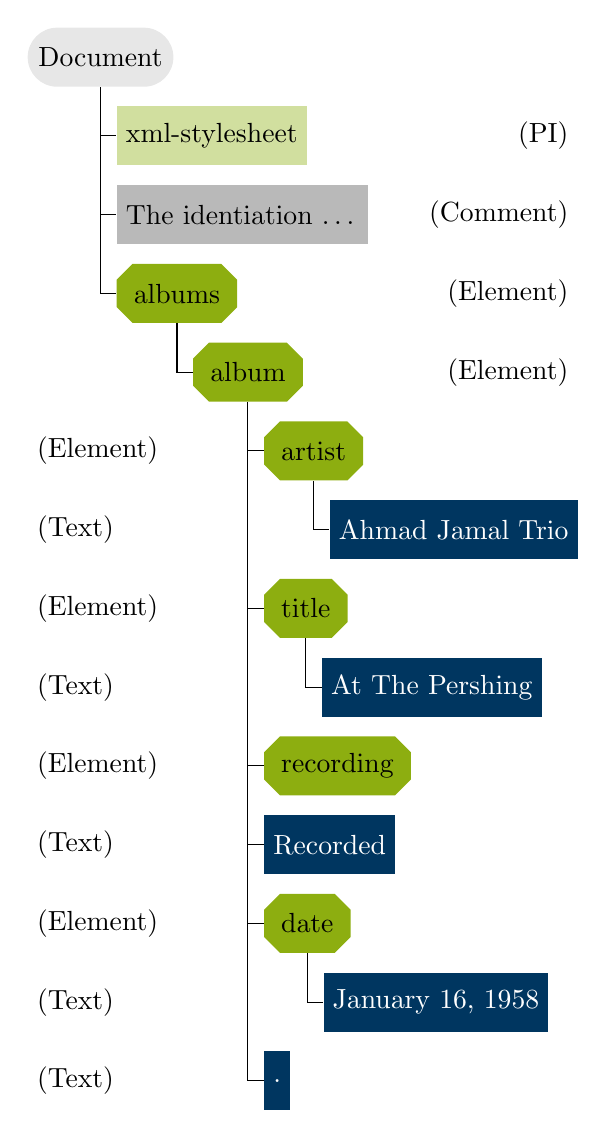
\begin{tikzpicture}
    \node [doc] (doc) {Document}
        child {  node [pi] (xmlstyle) {xml-stylesheet} }
        child {  node [comment] (comment) {The identiation \dots{}} }
        child {  node [element] (albums) {albums}
            child {  node [element] (album) {album}
                child {  node [element] (artist) {artist}
                    child {  node [textnode] (trio) {Ahmad Jamal Trio} }
                }
                child {  node [element] (title) {title}
                    child {  node [textnode] (pershing) {At The Pershing} }
                }
                child {  node [element] (recording) {recording} }
                    child {  node [textnode] (recorded) {Recorded } }
                    child {  node [element] (date) {date}
                        child {  node [textnode] (datetext) {January 16, 1958} }
                    }
                    child {  node [textnode]  (textdot){.} }
            }
        };
        \node [anchor=east] at (xmlstyle -| trio.east) (desc) {(PI)};
        \node [anchor=east] at (comment -| desc.east) {(Comment)};
        \node [anchor=east] at (albums -| desc.east) {(Element)};
        \node [anchor=east] at (album -| desc.east) {(Element)};
        \node [anchor=west] at (artist -| doc.west) (leftdesc) {(Element)};
        \node [anchor=west] at (trio -| leftdesc.west) {(Text)};
        \node [anchor=west] at (title -| leftdesc.west) {(Element)};
        \node [anchor=west] at (pershing -| leftdesc.west) {(Text)};
        \node [anchor=west] at (recording -| leftdesc.west) {(Element)};
        \node [anchor=west] at (recorded -| leftdesc.west) {(Text)};
        \node [anchor=west] at (date -| leftdesc.west) {(Element)};
        \node [anchor=west] at (datetext -| leftdesc.west) {(Text)};
        \node [anchor=west] at (textdot -| leftdesc.west) {(Text)};

\end{tikzpicture}
\end{document}

